\chapter{FG Nup aggregation under crowded conditions}\label{ch05}

Disordered proteins are often prone to aggregation, often causing disease, and the aggregation behavior of FG Nups is important to understand.  It is not clear what the aggregation state of Nups is within the pore or how their aggregation might play into nuclear transport \cite{things}.  \textit{In vitro}, many Nups spontaneously aggregate into amyoids over the course of a few hours, but there is evidence that this aggregation does not happen in the cellular environment \cite{frey07, Loren's paper}.  We investigated aggregation behavoir of an aggregation-prone Nup fragment in a number of different crowders.  Inert crowders such as PEG and PVP help mimic the extremely crowded cellular environment, but they may interact different with the protein than nonspecifically-binding crowders such as cell lysate or BSA.  We wanted to understand how different crowders affected the aggregation properties of Nups.

We used a 124-amino-acid fragment of the Nup Nsp1.  The FG-repeat segment of Nsp1 contains an aggregation-resistant portion (used as the basis for the FSFG peptide) as well as one that aggregates in buffer over the course of a few hours.  This aggregation-prone portion is the basis of the FG124 peptide used in the following aggregation experiments.

We used aggregation timecourses with thioflavin T as a readout, as well as fluorimetry, NMR, and x-ray scattering.  Our conclusion is something about the phenylalanines and how they behave differently in when crowded with PEG than with PVP (which also has an aromatic ring).


\section{Results}
\subsection{Thioflavin timecourses}

We analyzed aggregation dynamics using thioflavin T, a fluorophore whose excitation and emission maxima shift and which grows much brighter in the presence of thioflavin.  Samples containing FG124, crowding agent, and thioflavin T were incubated while shaking overnight in a 96-well plate and their fluorescence intensity recorded every ten minutes.  The resulting traces show a typical aggregation pattern, with a lag phase, burst phase, and saturation phase.

Thioflavin T (ThT) is a dye that grows much brighter when bound to amyloids.  Upon binding, its absorption maximum shifts from from 385 nm to 450 nm and it emission maximum from 445 nm to 482 nm \cite{picken12}.  Although ThT is a more reliable indicator of amyloids than other fluorescence methods, notably Congo red stain, it suffers from reproducibility problems.  There is no consensus on the mechanism of ThT binding to amyloids.  Some proposed mechanisms rely on the presence of ThT micelles, which form above a critical concentration of about 4 $\mu$M, while others advocate for avoiding micelles \cite{khurana05, groenning09}.  There is some evidence that amyloid fibrils can adsorb to the plastic surface of a multiwell plate, decreasing ThT fluorescence intensity as the fibrils mature \cite{murray13}.  Often in our timecourse experiments, the ThT fluorescence did reach a maximum and then decrease.  The fluorescence intensity also depends on the sample pH, an effect which we noticed in our timecourses.  Despite these challenges, thioflavin T is the most consistent dye for detecting the process of amyloid formation.

The final concentration of crowding agent was 19\% serine w/v, 13\% PEG, and 13\% PVP.  Lysate concentration varied between time courses and was in the 1-10 mg/mL range.  Two timecourses were run with varying PEG and PVP concentrations: 25\%, 20\%, 13\%, and 5\%.  Samples with no crowding agent ('buffer" samples) were run as a reference, and samples in 7M guanidine hydrochloride (GuHCl) with no crowding agent were run as negative controls in each timecourse.  No aggregation was observed in the GuHCl samples.  In every case, blanks were run alongside the sample conditions.  In the blanks, the FG124 was omitted.

First the data were normalized to the blanks.  In nearly all cases, the blank intensity remained steady over time, as expected.  In those cases, the mean blank intensity was subtracted from the corresponding data.  (In cases where the blank intensity changed over time, it was subtracted pointwise from the data.)

Then the normalized curves were fit to a sigmoid given by
\begin{equation}
I(t) = C + \frac{A}{1+\exp \left(-k(t-T_{1/2})\right)}
\label{eq:fit}
\end{equation}
where $I(t)$ is the normalized fluoresence intensity as a function of time.  The useful physical parameters for our purposes are the time constant $k$, which gives a measurement of the steepness of the slope at the beginning of the burst phase, and the lag time $T_l$.  The lag time is calculated as
\begin{equation}
T_l = T_{1/2} - \frac{2}{k}
\end{equation}
and represents the duration of the lag phase \cite{}.  

\begin{figure}
\caption{Sample sigmoid fit. Look up conditions.  (Pulled this from Sophie's thesis but I did the fit)}
\centering
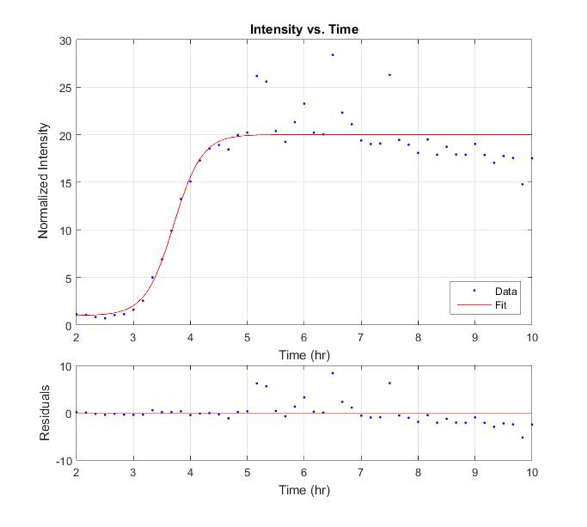
\includegraphics[width=0.5\textwidth]{figs/ch05/sigmoid-fit}
\label{fig:sigmoid-fit}
\end{figure}

Ideally, we expect $C=1$, as aggregation should not have begun at the start of the experiment, so there should be no increase in sample fluorescence over that of the blank.  Experimentally, $C$ usually ranged between 1 and 2, up to about 10 for some sample conditions.  This might have been because aggregation had already begun, but this seems unlikely because the lag phase continued for some time.  I don't know why  $C$ wasn't close to unity for all conditions and replicates.

The saturation phase asymptotes to an intensity given by $I_\tx{sat}=C+A$.  We found significant variation in $I_\tx{sat}$ for the same condition between timecourses, and the relative magnitudes of different conditions also varied between timecourses.  I think this is a limitation of the thioflavin tests.  Therefore, we do not consider $I_\tx{sat}$ in our analysis, leaving $k$ and $T_l$ as parameters of interest.

Next we normalized once again to account for differences between timecourses.  It was impossible to hold the concentration exactly fixed between timecourses, and there were probably some other environmental variables we couldn't control perfectly, so it was important to normalize again.  Within each timecourse, we averaged the fit parameters for all buffer replicates and subtracted that average from each other replicate.

\begin{figure}
\caption{test}
\centering
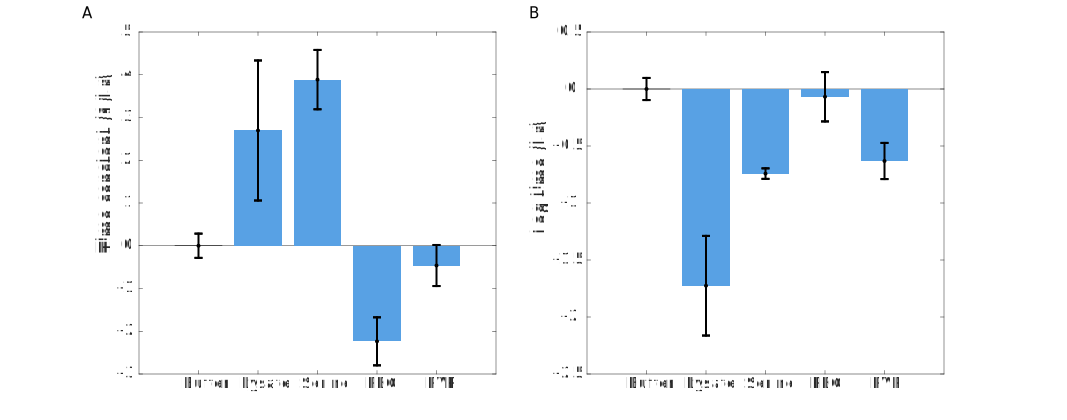
\includegraphics[width=\textwidth]{figs/ch05/barCharts}
\label{fig:fitParams}
\end{figure}

We then combined replicates from all timecourses by condition and took the final average and standard error of the mean for both fit parameters.  The results are shown in Fig.~\ref{fig:fitParams}.  I ran a one-factor ANOVA to reject the null hypothesis that all means were the same, and then two-sample t-tests on each pair of conditions to find which differences were statistically significant.  For the time constant, all pairs of conditions were significantly different from each other with $p < 0.05$ \emph{except} buffer-PVP.   For the lag time, all pairs of conditions were significantly different from each other with $p < 0.05$ \emph{except} buffer-PEG and serine-PVP.

\begin{figure}
\caption{test}
\centering
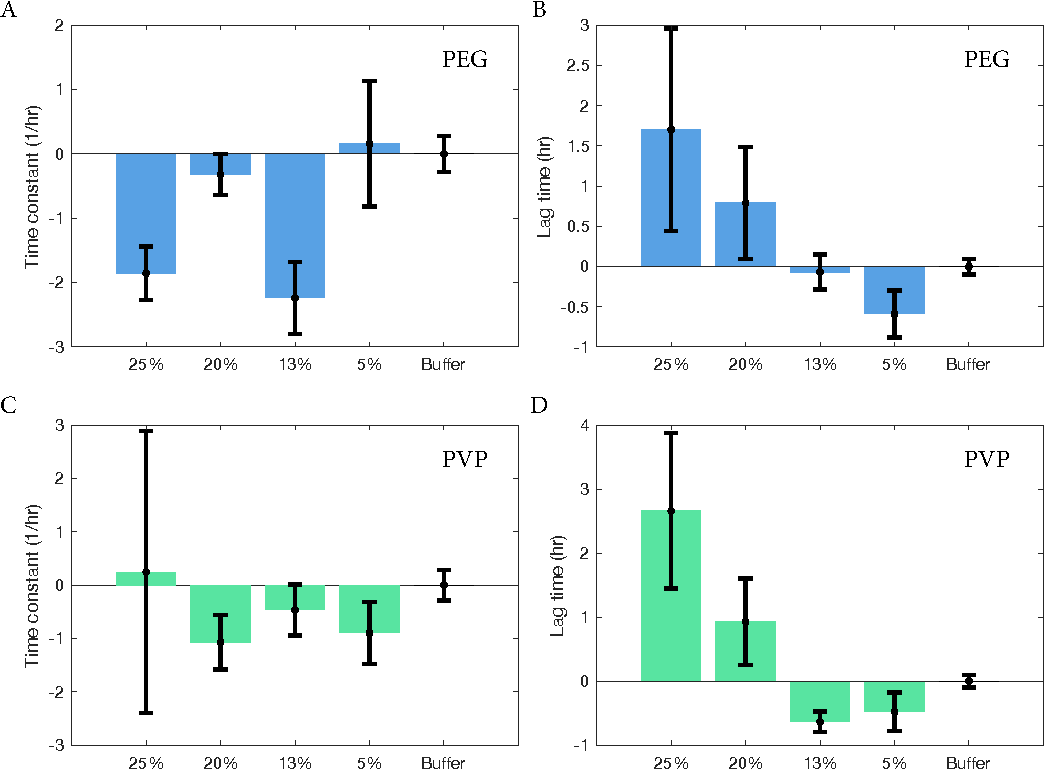
\includegraphics[width=\textwidth]{figs/ch05/peg-and-pvp-charts}
\label{fig:peg-pvp}
\end{figure}

I followed the same process for the timecourses involving the concentration series for PEG and PVP, but there were fewer significant differences between concentrations, as seen in Fig.~\ref{fig:peg-pvp}.  The ANOVA for the PEG time constants gave $p=0.0024$ with the t-test showing differences between: buffer-25\% PEG, buffer-13\% PEG, and 25\% PEG-20\% PEG. The ANOVA for the PEG lag times was likewise significant with $p = 0.0102$.  The significant pairs were: buffer-25\% PEG, buffer-20\% PEG, buffer-5\% PEG, and 25\% PEG-13\% PEG.

For PVP, there were no significant differences in the time constant.  For the lag time, after the ANOVA and t-tests, there were differences between: buffer and everything except 5\% PVP, 25\% PVP and everything but 20\% PVP, and 20\%PVP-13\% PVP.

For both conditions, it looks roughly like the lag time increases with the crowder concentration, but given the large error bars, I wouldn't read too much into it.  The time constants don't follow any particular trend and are mostly indistinguishable anyway.

We tested the effects of pH on FG124 aggregation by running several experiments in buffer at varying pH.  We ran six replicates of each condition, for pH values between 5 and 8.  No significant differences were found in the lifetimes or lag times of any pH condition.  Results are summarized in Table \ref{table:FG124-pH}. We concluded that aggregation is not affected by pH in the range 5-8.

\begin{table}[b!]
  \caption{FG124 aggregation lifetime and lag time with varying pH. Each condition run with 6 replicates in PTB buffer.  One-way ANOVAs show no statistically significant differences between conditions.  Standard errors are shown.}
    \label{table:FG124-pH}
    \begin{tabular}{p{1cm}p{3cm}p{3cm}}
      pH & Lifetime $\tau$ (hr) & Lag time $T_{lag}$ (hr) \\
      \hline
      5 & $0.34 \pm 0.09$ & $6.8 \pm 0.1$ \\
      6 & $0.35 \pm 0.12$ & $6.2 \pm 0.2$ \\
      7 & $0.38 \pm 0.14$ & $6.8 \pm 0.4$ \\
      8 & $0.50 \pm 0.14$ & $6.6 \pm 0.2$ \\
    \end{tabular}
\end{table}
\subsection{Fluorimetry}
We hypothesized that the crowder-dependent difference in aggregation might arise from the aromatic ring in PVP, which could interact with the phenylalanine in FG124 in a ring-stacking interaction.  To test this idea, I collected emission spectra of fresh and aggregated FG124 in PEG and PVP crowders near the phenylalanine peak wavelength (see Fig. \ref{fig:FG124-fresh-vs-agg}).  Only 5\% PEG and PVP in PTB were tested because PEG has a peak near the FG124 peak which dominates at higher PEG concentrations.  Data were normalized by averaging over two runs and subtracting a blank run (containing crowder and buffer but no protein).
\begin{figure}
\caption{Emission scan of fresh and aggregated FG124 in crowded conditions.  Data normalized by subtracting blank sample.}
\centering
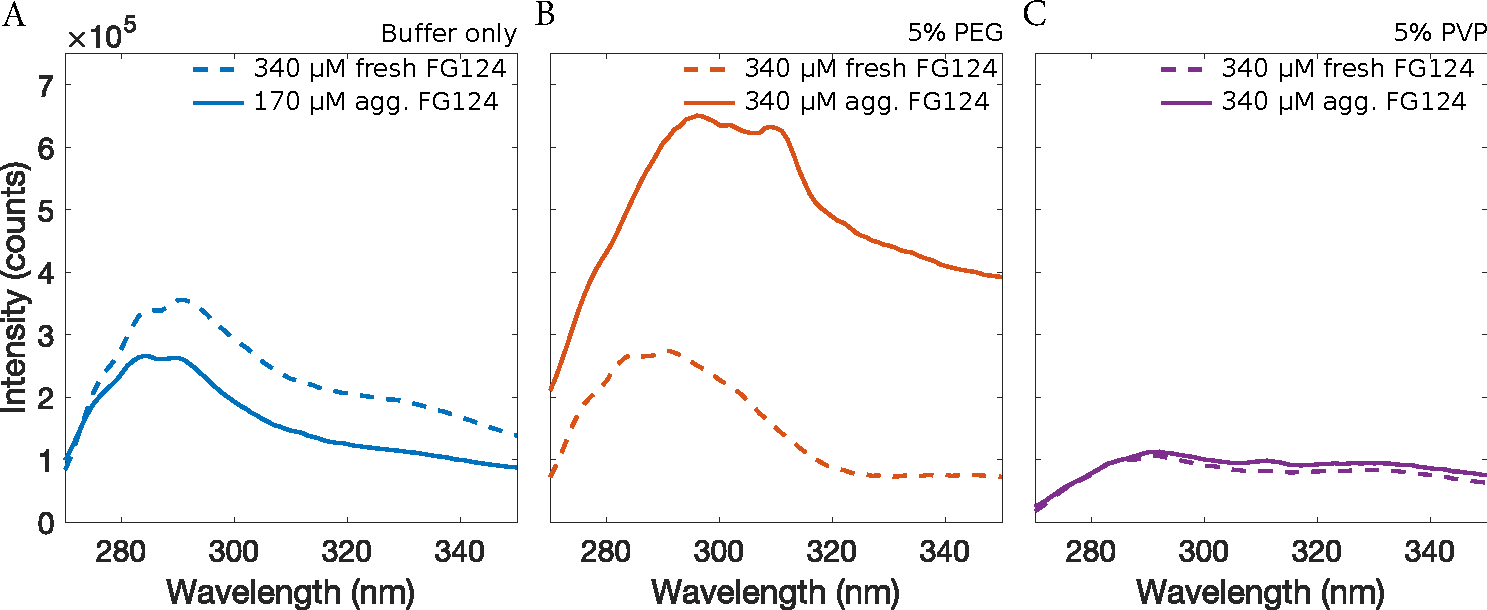
\includegraphics[width=1.1\textwidth]{figs/ch05/FG124-fresh-vs-agg}
\label{fig:FG124-fresh-vs-agg}
\end{figure}
The PEG sample showed the largest difference upon aggregation, both in peak height and location.  Figure \ref{fig:stacked-FG124-fluorimetry} shows the same data, normalized to a maximum amplitude of one and offset, in order to emphasize the changes in peak shape.
\begin{figure}
\caption{Emission scan of phenylalanine, FSFG, and FG124. Excited at 240 nm.  Phe data is not mine, need to check reference. Data normalized to a maximum amplitude of 1.}
\centering
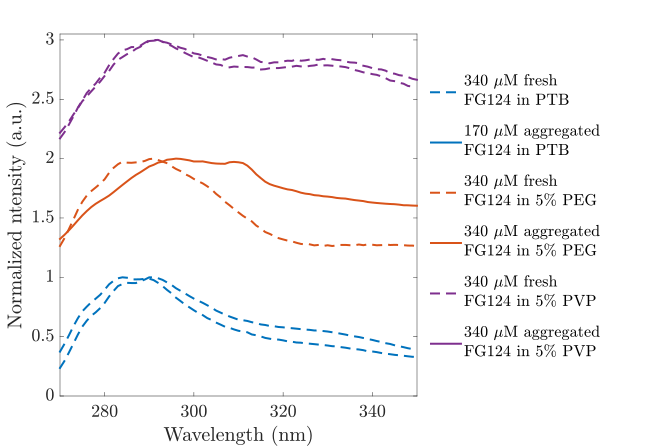
\includegraphics[width=\textwidth]{figs/ch05/stacked-FG124-fluorimetry}
\label{fig:stacked-FG124-fluorimetry}
\end{figure}
In both crowder conditions, but not in the buffer condition, a small peak appears in the aggregated FG124 near 310 nm.

Additionally, I compared the phenylalanine peaks in FSFG and fresh and aggregated FG124 to those of pure phenylalanine \cite{zotero-5177}, as seen in Fig. \ref{fig:phe-comparison}.  Data are blanked and normalized to a maximum intensity of one.  The peak slightly shifts toward longer wavelengths as the data progress from phenylalanine to FSFG to fresh and aggregated FG124.
\begin{figure}
\caption{Emission scan of phenylalanine, FSFG, and FG124. Excited at 240 nm.  Phe data is not mine, need to check reference. Data normalized to a maximum amplitude of 1.}
\centering
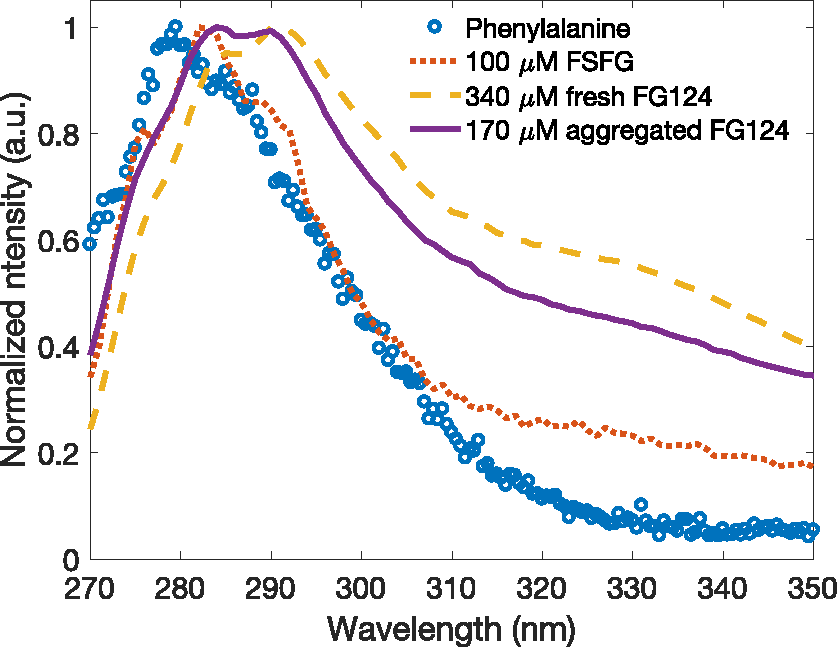
\includegraphics[width=0.5\textwidth]{figs/ch05/phe-comparison}
\label{fig:phe-comparison}
\end{figure}
I also measured PEG and PVP absorbance near 240 nm (see Fig.~\ref{fig:crowder-absorbance}).  PVP has a very high absorbance in that range, which might explain why the recorded counts were lowest for the PVP conditions.
\begin{figure}
\caption{Absorbance of 5\% PEG and PVP solutions in PTB.  Normalized by subtracting PTB absorbance.}
\centering
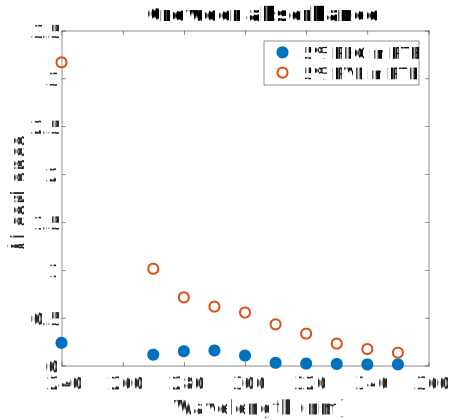
\includegraphics[width=0.5\textwidth]{figs/ch05/crowder-absorbance}
\label{fig:crowder-absorbance}
\end{figure}

\section{Discussion}

It's possible that the differences in aggregation time between PEG and PVP come from changes in viscosity.  The two samples do have widely different viscosity, as measured by Steve Whitten.  A 13\% PEG solution in PTB has a dynamic viscosity of 15.87 mPa s, while that of a 13\% PVP solution in PTB is 7.34 mPa s.  The literature doesn't entirely agree on what happens to aggregation as a function of viscosity, but what we see could be due to that change.  (Check in lab book where I have lit search notes.)

\section{Materials and Methods}
\subsection{Buffers} Potassium transport buffer (PTB) (150 mM KCl, 20 mM HEPES, 2 mM $\tx{MgCl}_2$) was used for all timecourse and NMR samples.
\subsection{FG124 preparation} His-tagged FG124 was expressed in \emph{E. coli} in the plasmid pRSF.  Cultures were grown in LB and  induced at 37 degrees C for 2-4 hr with 1 mM IPTG at OD 0.6-0.8.  Periplasmic matrix was removed prior to lysis.  Cells were then lysed via sonication and FG124 purified using TALON cobalt resin.  All purification buffers were PTB with 7M GuHCl and PIC.  The elution buffer also contained 250 mM imidazole.
\subsection{Timecourse preparation} Stocks of PEG and PVP in PTB were prepared at 20 or 40\% w/v; serine stocks were prepared at 30\% w/v.  PEG and serine were at pH 7; PVP was pH 7 or pH 5.  A pH series with no crowding agent showed no significant differences based on pH.  Lyophilized lysate was prepared by homogenizing BL21 DE3 Gold cells and spinning them down.  The supernatant was lyophilized in a decomposing ammonium bicarbonate buffer and resuspended in PTB to the desired concentration when needed.  A 10 mM stock solution of ThT in PTB was prepared and filtered no more than a week before the timecourse, stored at room temperature and protected from light.  Immediately prior to starting the timecourse, FG124 was desalted into PTB to remove the imidazole and GuHCl.  Samples were promptly prepared containing the appropriate percentage of crowder, a final concentration of 1-2 mg/mL FG124, and 200 uM thioflavin T.  All samples in the same timecourse had the same concentration of FG124, including the buffer sample, which contained no crowding agent.  Blanks were prepared with crowding agent and thioflavin T, but no FG124.  Samples were pipetted into black, flat-bottomed, clear-bottomed 96-well plates with 150 uL per replicate.  Each sample yielded four to six replicates.  Only one blank replicate was used per condition.  One negative control and corresponding blank were prepared per timecourse containing 7M GuHCl and no crowding agent but using the same protein sample as all other conditions.  Each well contained a 3mm-diameter glass or teflon bead.  The plate was sealed with a PCR seal and taken to a Safire II plate reader.  The fluoresence was measured from the bottom at 10-minute intervals with an excitation wavelength of 450 nm, emission wavelength of 482 nm, and 5 nm bandwidths.  The plate shoook orbitally at high speed between measurements and was held at a temperature of 30 degrees C.  The time between desalting and beginning the plate reader measurements was typically about an hour; the time of desalting was taken as $t=0$ for the purposes of calculating lag time. In parallel with the sample preparation, the concentration of the desalted FG124 was measured with a BCA assay.
\subsection{NMR sample preparation}
\subsection{NMR experiments}
\subsection{Fluorimetry}

FG124 was purified as described above and stored in PTB with 7M GuHCl.  Immediately before use, 130 uL of 520 uM FG124 was desalted with a Zeba spin desalting column to remove the GuHCl.  The resulting stock was used in the crowder samples, which had a final concentration of 340 uM Fg124.  I used the shared-instrumentation fluorimeter.  I tested PTB, 5\% PEG (MW, source, purity?) in PTB, and 5\% PVP (same questions?) in PTB as blanks.  I measured 340 uM FG124 in PTB and the two crowders as well.  Between runs, I cleaned the cuvette (micro quartz cuvette from Kaar lab (sample volume?)) with ethanol 3x, then 5x with DI water, and gently blotted the outside with ethanol.  Fluorimeter settings: 4 nm slits, 1000 V PMT, excitation wavelength of 240 nm.  Step size  = 1nm, average over 2 runs.  After taking this data with fresh FG124, I let the samples sit at room temp overnight to aggregate (no shaking) and most were cloudy in the morning.  I took similar data with the aggregated samples.  I needed to rinse with 7M GuHCl, let soak in 7M GuHCl for 5 minutes, and then perform the same cleaning procedure as the previous day in order to remove the aggregates from the cuvette.

